\section{Fundamentos e Trabalhos Relacionados}\label{sec:fund-trabs-rel}

Esta seção reúne os fundamentos teóricos e os trabalhos relacionados que sustentam o desenvolvimento deste estudo, abordando os conceitos essenciais sobre labirintos, LLMs, estratégias de fine-tuning e métodos de explicabilidade.

\subsection{Labirintos e Raciocínio Espacial}

Labirintos são estruturas clássicas amplamente utilizadas para investigar processos de raciocínio espacial, planejamento e navegação, especialmente no contexto de agentes artificiais \cite{vartak2023mazesolverrobot}. Conceitualmente, um labirinto pode ser definido como um ambiente composto por caminhos interconectados, obstáculos e pontos de decisão, cujo objetivo é encontrar uma rota eficiente entre um ponto de entrada e um de saída. A resolução de labirintos demanda a construção de representações espaciais internas, identificação de padrões e adaptação de estratégias a partir da estrutura do ambiente, como \cite{sadik2010comprehensive} aborda comparando diferentes técnicas baseadas em teoria dos grafos.

Neste trabalho, labirintos em ASCII são empregados como um domínio controlado para testar a capacidade de modelos de linguagem em desenvolver representações espaciais e estratégias de navegação a partir de entradas exclusivamente textuais. Essa escolha permite investigar, com o apoio de técnicas de explicabilidade, se os modelos são capazes de realizar raciocínio estrutural coerente ou se apenas se baseiam em padrões estatísticos superficiais.

\subsection{LLMs - Large Language Models}

Os LLMs representam um marco no avanço do Processamento de Linguagem Natural (PLN), resultado de uma trajetória que abrange: modelos estatísticos, como n-gram; passando por modelos baseados em \textit{word embeddings}, como Word2Vec \cite{mikolov2013distributed}; \textit{Recurrent Neural Networks} (RNNs) e \textit{Long Short-Term Memory} (LSTM) \cite{hochreiter1997long} e, mais recentemente, arquiteturas baseadas em \textit{transformers} \cite{jurafsky2025slp3}.

\subsubsection{Arquitetura Transformer e Mecanismo de Atenção}

O desenvolvimento dos LLMs está diretamente ligado à evolução dos transformers, introduzidos por \cite{vaswani2023transformers}, que revolucionaram o campo ao permitir a modelagem eficiente de dependências contextuais de longo alcance, por meio de mecanismos de atenção. Sua arquitetura é composta por blocos de \textit{encoder} e \textit{decoder}, que podem ser utilizados separadamente ou em conjunto, conforme a tarefa. A figura \ref{fig:transformer-architecture} ilustra a arquitetura básica de um transformer, destacando seus componentes principais.

\begin{figure}[h!]
    \centering
    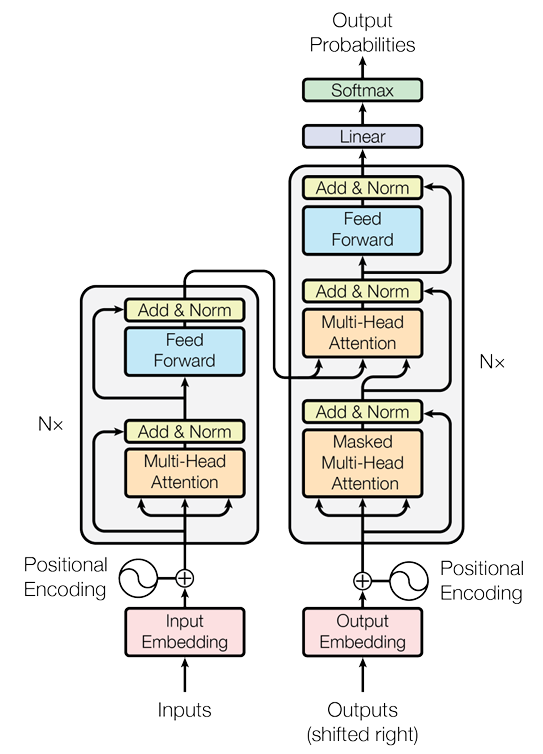
\includegraphics[width=0.39\textwidth]{figure/transformer-architecture.png}
    \caption{Arquitetura básica de um transformer, com blocos de encoder e decoder \cite{vaswani2023transformers}.}
    \label{fig:transformer-architecture}
\end{figure}

Modelos recentes, como o BERT \cite{devlin2019bert}, utilizam apenas o encoder, sendo eficazes em tarefas de compreensão textual, enquanto modelos GPT \cite{yenduri2023gpt} utilizam apenas o decoder, focando na geração de texto. Arquiteturas encoder-decoder, como o T5 \cite{raffel2023t5}, são empregadas em tarefas de tradução e sumarização \cite{tunstall2022nlptransformers}.

\subsubsection{Pré-treinamento e fine-tuning}

O treinamento dos LLMs ocorre em duas etapas principais: pré-treinamento e ajuste fino (\textit{fine-tuning}). No pré-treinamento, os modelos são expostos a grandes volumes de dados textuais não rotulados, aprendendo representações linguísticas gerais por meio de tarefas como predição de palavras mascaradas ou geração de texto \cite{tunstall2022nlptransformers}. Essa etapa é fundamental para fornecer aos modelos capacidades de compreensão e geração de linguagem \cite{zhao2025surveyllms}. O \textit{fine-tuning}, abordado em seção específica deste trabalho (\ref{sec:fund-finetuning}), permite especializar o modelo para tarefas ou domínios específicos.

\subsubsection{Modelos Atuais}

LLMs modernos, como GPT-3 \cite{brown2020languagemodelsfewshotlearners}, GPT-4 \cite{openai2024gpt4technicalreport}, PaLM \cite{chowdhery2022palmscalinglanguagemodeling} e outros, possuem bilhões de parâmetros e apresentam habilidades emergentes, incluindo raciocínio, compreensão semântica e adaptação a múltiplos contextos. No entanto, estudos e bibliografias recentes evidenciam limitações importantes desses modelos, como a propensão a respostas não factuais, vieses sociais e dificuldades em tarefas que exigem raciocínio profundo ou conhecimento de mundo \cite{chang2024lmsurvey, summerfield2025strange}.

Além dos LLMs tradicionais, surgiram variantes especializadas, como os Large Reasoning Models (LRMs) que incorporam mecanismos de raciocínio explícito \cite{lynch2025reasoning}, e os Multimodal Vision Language Models (VLMs) \cite{li2025surveystateartlarge}, que integram texto e imagens para tarefas multimodais. Essas alternativas buscam superar limitações dos LLMs convencionais e ampliar o espectro de aplicações dos modelos de linguagem.

\subsection{Fine-tuning de LLMs}\label{sec:fund-finetuning}

O \textit{fine-tuning} é uma etapa fundamental para adaptar LLMs a tarefas específicas, permitindo que modelos previamente treinados em grandes volumes de dados textuais sejam ajustados para contextos e domínios particulares. Neste trabalho, destacam-se duas estratégias principais: o \textbf{Supervised Fine-Tuning (SFT)} e o \textbf{Group Relative Policy Optimization (GRPO)}.

O \textbf{SFT} consiste no ajuste supervisionado do modelo utilizando conjuntos de dados rotulados, nos quais o modelo aprende a associar instruções ou entradas a saídas desejadas. Essa técnica é amplamente empregada para especializar LLMs em tarefas como classificação, tradução e, no contexto deste estudo, navegação em labirintos ASCII. O processo envolve a construção de um dataset de pares (instrução, saída) e o treinamento supervisionado para minimizar o erro entre a resposta do modelo e a resposta esperada \cite{zhang2024instructiontuning}. O SFT é considerado eficiente, pois permite adaptar rapidamente o modelo a novos domínios sem a necessidade de re-treinamento completo.

Já o \textbf{GRPO} é uma técnica baseada em otimização de políticas relativas a grupos, utilizada para aprimorar o desempenho do modelo considerando preferências coletivas de múltiplos usuários ou agentes. No GRPO, o modelo é ajustado para maximizar a satisfação de critérios definidos por grupos, promovendo respostas mais alinhadas a contextos colaborativos ou multiusuário \cite{dao2025alphamaze}. Essa abordagem é especialmente relevante em cenários onde a diversidade de preferências e estratégias é importante para o sucesso da tarefa.

Essas estratégias são relevantes para o presente estudo, pois permitem investigar como diferentes métodos de ajuste podem impactar o desempenho dos LLMs em tarefas de raciocínio espacial.

\subsection{Explicabilidade em LLMs}

Apesar do alto desempenho, LLMs são frequentemente criticados por seu caráter de “caixa-preta”, dificultando o entendimento sobre como tomam decisões e levantando preocupações éticas e de confiança \cite{zhao2023explainability, cambria2024xai, luo2024fromunderstanding}. A opacidade desses modelos pode resultar em respostas inesperadas, enviesadas ou até mesmo em alucinações, o que reforça a necessidade de técnicas de explicabilidade (\textit{explainability}) para tornar seus mecanismos internos mais transparentes.

A explicabilidade em LLMs pode ser abordada sob diferentes perspectivas. Do ponto de vista do usuário final, explicações claras e acessíveis são essenciais para promover confiança e permitir o uso responsável dos modelos em aplicações sensíveis, como saúde, educação e finanças. Para pesquisadores e desenvolvedores, a explicabilidade atua como ferramenta de diagnóstico, facilitando a identificação de vieses, falhas e oportunidades de aprimoramento dos modelos \cite{zhao2023explainability, luo2024fromunderstanding}.

As principais técnicas de explicabilidade para LLMs incluem métodos de atribuição de importância a tokens (feature attribution), análise de camadas internas, visualização de mecanismos de atenção e explicações baseadas em exemplos. Recentemente, abordagens baseadas em prompts e cadeias de raciocínio (\textit{chain-of-thought} \cite{wei2023chainofthought}) também têm sido exploradas para tornar o processo de decisão dos modelos mais interpretável \cite{zhao2023explainability}. No entanto, o aumento da escala e da complexidade dos LLMs impõe desafios adicionais, tornando a geração de explicações confiáveis e compreensíveis uma tarefa ainda em aberto.

Além disso, a literatura destaca a importância de desenvolver métricas e benchmarks específicos para avaliar a qualidade das explicações geradas, bem como de promover a integração entre avanços em LLMs e técnicas de XAI (Explainable AI) \cite{cambria2024xai}. O avanço conjunto dessas áreas é fundamental para garantir o uso ético, seguro e transparente dos modelos de linguagem em aplicações reais.

\subsubsection{LLM-MRI}

A biblioteca LLM-MRI (\textit{Large Language Model - Magnetic Resonance Imaging}) é uma ferramenta desenvolvida para facilitar a análise de padrões de ativação em LLMs baseados em \textit{transformer}. Conforme apresentado por \cite{costa2024llmmri}, a LLM-MRI permite coletar, organizar e projetar em dimensões reduzidas os vetores de ativação gerados pelos modelos ao processarem diferentes entradas. Técnicas de redução de dimensionalidade possibilitam visualizar como as ativações neuronais se distribuem, facilitando a identificação de padrões e a análise das mudanças provocadas por diferentes estratégias de fine-tuning.

No contexto deste trabalho, a LLM-MRI é empregada para investigar como LLMs se adaptam à tarefa de navegação em labirintos ASCII e como as estruturas internas dos modelos evoluem durante o processo de aprendizagem, contribuindo para a análise da interpretabilidade e do raciocínio espacial dos modelos.
\subsection{Trabalhos Relacionados}

Esta seção apresenta a revisão de literatura sobre o tema deste trabalho, com foco em LLMs, fine-tunning e explicabilidade.

\subsubsection{Labirintos como Domínio Estrutural para Raciocínio Espacial}

A investigação do raciocínio espacial em modelos de linguagem tem utilizado labirintos como um domínio estruturado e simbólico, capaz de revelar limitações e padrões de generalização dos modelos. O benchmark introduzido por \cite{zhou2024navigatingshortcutmazecomprehensive}, avalia a suscetibilidade dos LLMs a se apoiarem em atalhos (\textit{shortcuts}) superficiais, ou correlações onde não há relação de causa-efeito, que afetam a robustez dos modelos em tarefas de classificação de texto.

Em outra abordagem, \cite{hsu2025whatmakesmazelooklike} propuseram o framework Deep Schema Grounding (DSG), que utiliza LLMs para extrair e estruturar representações simbólicas (schemas) do conceito de labirinto, promovendo um raciocínio mais alinhado à cognição humana ao combinar essas abstrações com modelos multimodais. Essas contribuições reforçam a relevância dos labirintos textuais como ambiente de análise para o comportamento de LLMs em tarefas que exigem planejamento, abstração e robustez interpretativa.

\subsubsection{Raciocínio Espacial em LLMs}

O raciocínio espacial em LLMs tem sido explorado por diferentes abordagens, buscando adaptar esses modelos para tarefas que exigem compreensão e manipulação de ambientes estruturados.

O AlphaMaze \cite{dao2025alphamaze} propõe um processo em duas etapas: inicialmente, o modelo é ajustado via Supervised Fine-Tuning (SFT) para aprender comandos de movimentação em labirintos textuais; em seguida, utiliza-se o Group Relative Policy Optimization (GRPO) para aprimorar o raciocínio e a autocorreção. O MazeBench é empregado para avaliar o desempenho dos modelos em diferentes níveis de dificuldade, evidenciando ganhos após o GRPO.

Em paralelo, \cite{wang2024pictureworththousandwords} questionam a vantagem de modelos multimodais em tarefas espaciais, mostrando que LLMs baseados apenas em texto podem superar alternativas multimodais, o que reforça a relevância de investigar estratégias específicas para LLMs textuais. Em contextos tridimensionais, \cite{zhang2025doespointcloudboost} identificam limitações dos LLMs, enquanto \cite{cheng2024spatialrgpt} propõem integrar módulos de representação de regiões e informações de profundidade para melhorar a compreensão espacial.

Outras abordagens, como o Chain-of-Symbol (COS) Prompting \cite{hu2024chainofsymbol}, convertem descrições em linguagem natural para representações simbólicas intermediárias, otimizando o planejamento espacial e reduzindo o uso de tokens. Já o Visualization of Thought (VoT) \cite{wu2024visualizationofthought} estimula a geração de representações visuais em ASCII art, inspirando-se na cognição humana para melhorar o acompanhamento de estados e o planejamento de ações. Embora o VoT apresente avanços em determinados cenários, sua eficácia depende das habilidades emergentes dos modelos e da qualidade dos prompts, sendo limitado em tarefas mais complexas ou com modelos menos robustos.

Ainda, mesmo com avanços recentes, variantes como os LRMs, que incorporam mecanismos explícitos de raciocínio, como cadeias de pensamento (\textit{Chain-of-Thought} \cite{wei2023chainofthought}) e auto-reflexão, ainda enfrentam desafios em tarefas de alta complexidade, apresentando limitações na generalização e fenômenos como raciocínio redundante ou ineficiente \cite{shojaee2025illusionthinking}.

Por fim, no contexto deste trabalho, o raciocínio espacial é central, pois o objetivo é investigar como LLMs podem ser ajustados e analisados para resolver labirintos representados em ASCII. As abordagens discutidas na literatura fornecem subsídios para a escolha de técnicas de fine-tuning e avaliação, além de motivar o uso de ferramentas de explicabilidade para compreender como as representações internas dos modelos evoluem ao longo do treinamento.

\subsubsection{Fine-tuning de LLMs para Tarefas Específicas}

O fine-tuning de LLMs para tarefas específicas é um tema amplamente investigado, com diferentes estratégias sendo propostas para aprimorar a adaptação dos modelos. Por exemplo, \cite{jiang2024supervised} demonstra que o uso de SFT pode melhorar tanto as representações internas quanto a capacidade de generalização, mesmo em modelos visuais, evidenciando a importância do ajuste direcionado para tarefas de raciocínio espacial.

Além disso, \cite{hsieh2023distillingstepbystep} propõem a utilização de \textit{rationales} gerados por LLMs como supervisão adicional em um cenário multitarefa, combinando rótulos e explicações para enriquecer o sinal de treinamento. Essa abordagem, baseada em Chain-of-Thought prompting \cite{wei2023chainofthought}, permite que modelos menores alcancem desempenho superior a LLMs maiores, mesmo com menos dados, ao tornar o processo de ajuste mais eficiente e interpretável. No contexto deste trabalho, a integração de racionalizações se mostra relevante para aprimorar a eficiência e a interpretabilidade dos modelos.

\subsubsection{Explicabilidade em LLMs}

A explicabilidade em LLMs é um campo em expansão, com abordagens que buscam tornar os modelos mais transparentes e compreensíveis. A biblioteca LLM-MRI \cite{costa2024llmmri} destaca-se por permitir a análise e visualização das ativações neuronais, facilitando a interpretação de como os modelos se adaptam a tarefas específicas.

Complementarmente, \cite{wu2025usablexai10strategies} propõem o conceito de Usable XAI, que enfatiza a aplicação prática das explicações para diagnóstico e aprimoramento dos modelos. Entre as estratégias discutidas estão métodos de atribuição, análise das ativações internas e explicações baseadas em exemplos, todas relevantes para entender a evolução das representações internas durante o fine-tuning. A integração dessas abordagens contribui para identificar limitações, corrigir vieses e aprimorar o desempenho dos modelos em tarefas que exigem alto grau de interpretabilidade.